%% IEEE journal draft for hierarchical JSSP-based intersection management.
\documentclass[journal]{IEEEtran}

\usepackage{cite}
\usepackage{graphicx}
\usepackage{amsmath}
\usepackage{amssymb}
\usepackage{bm}
\usepackage{array}
\usepackage{booktabs}
\usepackage{multirow}
\usepackage{siunitx}
\usepackage[caption=false,font=footnotesize]{subfig}
\usepackage{algorithmic}
\usepackage{url}
% \usepackage[hidelinks]{hyperref}
\usepackage{hyperref}
\usepackage{xcolor} % 提供颜色支持
\usepackage{soul}   % 提供高亮标注支持

\graphicspath{{assets/figures/}}
\DeclareGraphicsExtensions{.pdf,.png,.jpg,.jpeg}

\hypersetup{
  pdftitle={Hierarchical JSSP-Based Scheduling With Smooth Trajectory Optimization for Autonomous Intersection Management},
  pdfauthor={Author Name},
  pdfkeywords={autonomous intersection management, job shop scheduling, reinforcement learning, trajectory smoothing, connected autonomous vehicles}
}

\hyphenation{op-tical net-works semi-conduc-tor sched-ul-ing tra-jec-to-ry}

\begin{document}

\title{Hierarchical JSSP-Based Scheduling With Smooth Trajectory Optimization for Autonomous Intersection Management}

\author{Author~Name%
\thanks{Author information, affiliation, and funding acknowledgment will be updated before submission.}%
\thanks{Manuscript prepared as an IEEE journal-style draft.}}

\markboth{IEEE Journal Draft,~2026}%
{Author: Hierarchical JSSP-Based Scheduling With Smooth Trajectory Optimization}

\maketitle

\begin{abstract}
% EN: Write one compact paragraph after the main method and results become stable. Mention the problem, method, validation platform, and main quantitative gains.
% CN: 摘要最终需要包含研究问题、核心方法、验证平台和关键定量结果。现在先保留轻量英文骨架，等实验完成后替换数字。
Autonomous intersection management can improve traffic efficiency when connected autonomous vehicles communicate through V2V and V2X channels, but a schedule that is optimal at an abstract conflict-zone level is not automatically executable by real vehicles. This paper proposes a hierarchical framework that formulates intersection passing order as a job shop scheduling problem and learns a high-level scheduler with reinforcement learning. \addedtwo{The target intersection is represented as $\mathcal{I}=(\mathcal{Z},\mathcal{T})$, where conflict zones and admissible route templates are transformed into an operation graph for relation-aware attention-based policy rollout.} The scheduled conflict-zone entry times are then passed to a low-level trajectory smoother that adjusts vehicle speed in advance, reducing unnecessary stops before the intersection while preserving safety constraints. The framework is designed for event-triggered replanning in SUMO and future vehicle-in-the-loop validation in CARLA. The expected outcome is an intersection manager that combines the global ordering strength of graph-based JSSP scheduling with smoother, more energy-aware vehicle motion.

\end{abstract}

\begin{IEEEkeywords}
Autonomous intersection management, connected autonomous vehicles, job shop scheduling problem, reinforcement learning, trajectory optimization, velocity smoothing, V2X.
\end{IEEEkeywords}

\IEEEpeerreviewmaketitle

\section{Introduction}
\label{sec:introduction}
% CN-SECTION: 引言说明研究背景、核心gap、本文层次化方案和贡献。
% EN: Start from the real-world need: AVs, logistics yards, warehouses, ports, and urban intersections. Then narrow to the gap between high-level schedules and low-level vehicle execution.
% CN: 先写现实背景：自动驾驶、智能工厂、仓库、港口和城市路口。然后逐步收束到本文关注的核心 gap：调度结果如何被车辆平滑执行。

\IEEEPARstart{A}{utonomous} vehicles are increasingly deployed in structured environments such as intelligent factories, warehouses, and ports, while connected autonomous vehicles are also becoming more relevant for urban traffic systems. With vehicle-to-vehicle and vehicle-to-infrastructure communication, an intersection no longer needs to be controlled only by fixed signal phases or human driving conventions. Instead, autonomous intersection management can coordinate the passing order of vehicles before they reach the conflict area.

Early scheduling methods often rely on predefined rules such as first-come-first-served policies, reservation mechanisms, or hand-designed heuristics. These methods are intuitive and easy to deploy, but their search space grows rapidly when traffic density increases and many vehicles compete for overlapping conflict zones. More recent graph-based and job-shop-scheduling-inspired formulations provide a compact way to represent the conflict relationship between vehicles and intersection zones.

However, a high-quality abstract schedule is only one part of the control problem. After a vehicle receives an assigned passing order or scheduled conflict-zone time, it must still adapt its speed and acceleration to satisfy the schedule. If vehicles simply stop at the stop line and wait for their turn, the intersection may suffer from stop-and-go waves, longer delay, and higher energy consumption. A smoother velocity profile can reduce unnecessary stops and make the schedule more practical for real vehicle execution.

\begin{addedblock}
This paper bridges this gap by combining high-level JSSP-based scheduling and low-level trajectory smoothing. The high-level scheduler is trained offline and deployed online as a fixed policy: when a scheduling event occurs, the policy sequentially rolls out operation decisions until all remaining conflict-zone traversals of the active vehicles have been ordered. A schedule generator then converts the selected operation order into target conflict-zone entry times, which are passed to the low-level smoother for physically feasible execution.
\end{addedblock}

The main contributions are summarized as follows:
\begin{addedblock}
\begin{itemize}
  \item A hierarchical autonomous intersection management framework that connects JSSP-based passing-order optimization with vehicle-level trajectory execution.
  \item An event-triggered online rollout mechanism in which an offline-trained RL policy constructs the remaining operation order for the current active vehicle set.
  \item A low-level speed smoothing formulation that tracks scheduled conflict-zone times while reducing unnecessary stop-line waiting.
  \item A simulation-oriented evaluation plan comparing the proposed method with first-come-first-served, heuristic scheduling, and scheduler-only baselines.
\end{itemize}
Compared with studies that focus only on high-level ordering or only on low-level vehicle control, this paper explicitly studies the interface between graph-based JSSP scheduling and executable smooth trajectories for autonomous intersection management.
\end{addedblock}

% CN summary for author review only; not visible in the compiled PDF:
% 本文强调高层调度器在线阶段不持续训练 RL，而是使用离线训练好的策略进行 sequential rollout，直到当前 active vehicles 的剩余冲突区操作全部排完，再将 order 和 target times 传给低层轨迹平滑器。
% EN: Add verified citations for FCFS, reservation-based AIM, JSSP-based AIM, stop-and-go energy loss, and smooth velocity planning.
% CN: 后续需要在这里补充真实引用：FCFS、预约式路口管理、JSSP 路口调度、停车波/能耗、速度平滑控制等。



\section{Related Work}
\label{sec:related_work}
% CN-SECTION: 文献综述按主题说明AIM、JSSP/RL调度和轨迹平滑的已有工作及不足。
% EN: Organize this section by research themes rather than paper-by-paper summaries. Each paragraph should end by explaining what limitation motivates this paper.
% CN: 本节建议按主题组织，而不是逐篇论文罗列。每个主题最后说明它和本文工作的差距。

\subsection{Autonomous Intersection Management}
% EN: Review signal-free AIM, reservation-based approaches, and centralized/decentralized coordination.
% CN: 回顾无信号灯路口管理、预约式方法、集中式和分布式协调方法。
Autonomous intersection management replaces fixed traffic signals with negotiated or optimized vehicle movements and has been widely discussed as a promising direction for connected autonomous traffic systems \cite{zhong2020autonomous}. Reservation-based approaches divide the intersection into spatial or temporal resources, while rule-based methods determine priority through arrival time, lane, or safety margins. These methods are practical baselines because they are interpretable and computationally light, but they may become conservative when traffic demand is high.

\subsection{Scheduling and Graph-Based Formulations}
% EN: Explain how conflict zones can be viewed as shared machines and vehicles as jobs. Discuss why JSSP is attractive for dense traffic.
% CN: 解释冲突区如何对应机器、车辆如何对应作业，并说明 JSSP 适合高密度交通的原因。
The job shop scheduling problem provides a natural abstraction for intersection coordination. Each vehicle can be treated as a job, each conflict zone as a machine, and each vehicle-zone traversal as an operation. Precedence constraints preserve the geometric order of zones along a path, while disjunctive constraints prevent two conflicting vehicles from occupying the same zone at the same time. This abstraction is attractive because it converts a traffic coordination problem into a structured combinatorial optimization problem.

\subsection{Reinforcement Learning for Combinatorial Scheduling}
% EN: Discuss RL policies that construct schedules step by step, including state, action, and reward design.
% CN: 讨论强化学习如何逐步构建调度序列，重点写状态、动作和奖励设计。
Reinforcement learning has been used to learn dispatching policies for combinatorial scheduling problems where handcrafted priority rules are difficult to tune. In a JSSP setting, an agent can observe the current partial schedule and select the next schedulable operation. For intersection management, this mechanism can be adapted to select which vehicle should enter a conflict zone next. The key challenge is to design an observation representation that captures safety, route order, and traffic density while remaining computationally efficient.

\begin{addedblock}
In the present framework, reinforcement learning is used to learn a constructive scheduling policy before deployment. During online intersection control, the trained policy parameters remain fixed, and the policy is queried repeatedly to complete the schedule for the active vehicle set. This distinction is important because online rollout has a clearer real-time role than continuous online training while vehicles are being controlled.
\end{addedblock}

\begin{addedtwoblock}
The proposed scheduler uses a relation-aware graph attention encoder because the operation graph contains typed structural relations: route-precedence edges, reverse route context, and same-zone disjunctive conflicts. This design is motivated by graph attention networks, relation-aware attention, relational graph neural networks, and learning-based JSSP dispatching on disjunctive graphs \cite{velickovic2018graphattention,shaw2018selfattention,schlichtkrull2018rgcn,chen2021rgat,zhang2020learningdispatch}.
\end{addedtwoblock}
\subsection{Trajectory Smoothing and Stop Avoidance}
% EN: Review velocity planning, energy-aware control, control barrier functions, and smooth crossing strategies.
% CN: 回顾速度规划、能耗优化、控制屏障函数和平滑通过路口的方法。
\begin{addedtodayblock}
Recent work shows that intersection efficiency depends not only on the discrete passing order but also on whether the assigned order can be executed by dynamically feasible vehicle trajectories. Graph-based CAV cooperation methods model crossing, diverging, converging, and reachability conflicts before selecting a passing order, which is close in spirit to representing conflict zones as shared scheduling resources \cite{chen2021conflictfree,chen2021lanechanging}. Priority-aware resequencing further shows that strict FCFS/FIFO decision orders can be relaxed through replanning while still passing target times to a lower-level optimal controller \cite{chalaki2021priority}. These studies motivate the scheduling layer in this paper, but they usually rely on handcrafted graph algorithms or analytic resequencing rather than an offline-trained graph policy.

Trajectory-level studies address the complementary question of how a vehicle should move after a desired crossing time, phase, or maneuver has been selected. Eco-driving and eco-approach controllers use reinforcement learning, Pontryagin-minimum-principle solutions, or hybrid rule-learning structures to reduce energy consumption, delay, and unnecessary acceleration near intersections \cite{bai2022hybrid,jiang2023ecodriving,lakshmanan2022cooperative,dong2023overtaking}. These papers support the use of stop count, acceleration variation, and energy proxy metrics in the evaluation, because stop-line waiting is not merely a delay phenomenon but also changes the smoothness and energy profile of the vehicle trajectory.

Safety-oriented trajectory planning adds constraints that the high-level schedule alone cannot guarantee. Predictive-control and spatial-domain formulations derive trajectories under rear-end, crossing, merging, diverging, and mixed-traffic uncertainty constraints \cite{mahbub2022safety,zhao2025spatial}. Learning-based AIM approaches can improve flexibility and travel time, but recent work also emphasizes that learned decisions need explicit safety evaluation or filtering, such as uncertainty-aware high-order control barrier functions \cite{luo2023realtime,yu2025uncertainty,cederle2024distributed,li2023dhal}. A broad CAV-control survey similarly identifies trajectory tracking, collaborative control, safety, comfort, and energy saving as coupled requirements rather than independent design goals \cite{liu2023systematic}.

The proposed framework follows this schedule-to-trajectory view. The high-level JSSP/RL scheduler determines the conflict-zone order and target entry times, while the low-level smoother treats those times as references to be tracked under speed, acceleration, jerk, and safety constraints. If the smoother cannot track the assigned reservations without violating collision-avoidance or comfort bounds, it reports infeasibility and triggers replanning or conservative stop-line fallback. This feedback interface is the main distinction from methods that optimize only the passing order or only the vehicle trajectory in isolation.
\end{addedtodayblock}

% EN: Before submission, ensure every cited claim has a verified source. Do not add placeholder citations.
% CN: 投稿前必须确认每个引用支撑相应论断，不要为了占位编造引用。





\section{Problem Formulation}
\label{sec:problem_formulation}
% CN-SECTION: 问题建模定义路口、车辆路线、JSSP映射、图结构、目标函数和安全假设。
% EN: Define the mathematical problem carefully. Keep notation consistent with the later scheduler and smoother sections.
% CN: 本节要严谨定义数学问题，并保证符号和后面的调度器、轨迹平滑部分一致。

\subsection{Intersection Conflict-Zone Model}
% EN: Describe how the intersection is divided into conflict zones and how each route maps to an ordered sequence of zones.
% CN: 写清楚路口如何划分冲突区，以及每条车辆路径如何对应一个有序冲突区序列。
Consider an intersection management region with a set of connected autonomous vehicles $\mathcal{V}$ and a set of conflict zones $\mathcal{Z}$. Each vehicle $i \in \mathcal{V}$ follows a known route through an ordered conflict-zone sequence
\begin{equation}
  \mathcal{R}_i = \left(z_{i,1}, z_{i,2}, \ldots, z_{i,n_i}\right), \quad z_{i,k} \in \mathcal{Z}.
\end{equation}
The route sequence is determined by the vehicle's incoming lane, outgoing lane, and turning movement.

\begin{addedtwoblock}
The target intersection is represented as a tuple
\begin{equation}
  \mathcal{I}=\left(\mathcal{Z},\mathcal{T}\right),
  \label{eq:intersection_tuple}
\end{equation}
where $\mathcal{Z}$ denotes the conflict-zone set and $\mathcal{T}$ denotes the admissible route or trajectory templates through the intersection. Each template in $\mathcal{T}$ induces an ordered sequence of zones and a nominal traversal model that can be used to estimate distance-to-zone, free-flow crossing time, and occupancy time.
\end{addedtwoblock}

\begin{figure}[!t]
\centering
\begin{tikzpicture}[
  font=\scriptsize,
  node distance=4mm,
  pblock/.style={draw=revisionpurple, rounded corners=1pt, align=center, text width=.86\linewidth, inner sep=2.8pt, text=revisionpurple, line width=.35pt},
  parr/.style={-{Stealth[length=1.8mm,width=1.2mm]}, draw=revisionpurple, line width=.35pt}
]
\node[pblock] (tuple) {Intersection tuple $\mathcal{I}=(\mathcal{Z},\mathcal{T})$};
\node[pblock, below=of tuple] (ops) {Operation nodes $v_{i,k}$: vehicle $i$ traverses zone $z_{i,k}$};
\node[pblock, below=of ops] (edges) {Edges: conjunctive route order $\mathcal{C}$ and disjunctive same-zone conflicts $\mathcal{D}$};
\node[pblock, below=of edges] (rollout) {Relation-aware policy rollout selects a feasible passing order};
\draw[parr] (tuple) -- (ops);
\draw[parr] (ops) -- (edges);
\draw[parr] (edges) -- (rollout);
\end{tikzpicture}
\caption{\addedtwo{Transformation from an intersection tuple to an operation graph for high-level scheduling.}}
\label{fig:intersection_tuple_graph}
\end{figure}

\subsection{JSSP Representation}
% EN: Explain vehicle-job, conflict-zone-machine, and traversal-operation mappings.
% CN: 解释车辆对应 job，冲突区对应 machine，车辆穿越冲突区对应 operation。
The intersection scheduling problem is formulated as a job shop scheduling problem. Vehicle $i$ is treated as a job $J_i$, conflict zone $z$ is treated as a machine $M_z$, and the traversal of vehicle $i$ through zone $z_{i,k}$ is an operation $O_{i,k}$. Each operation has a processing time $p_{i,k}$ that approximates the time required for vehicle $i$ to occupy and clear conflict zone $z_{i,k}$.

\begin{addedtwoblock}
For the neural scheduler, the active scene is converted into an operation graph
\begin{equation}
  \mathcal{G}=\left(\mathcal{V}_g,\mathcal{C}\cup\mathcal{D}\right),
  \label{eq:operation_graph}
\end{equation}
where $\mathcal{V}_g=\{v_{i,k}\mid i\in\mathcal{V}, z_{i,k}\in\mathcal{R}_i\}$ is the set of operation nodes. The graph-node notation $\mathcal{V}_g$ is used to avoid confusion with the vehicle set $\mathcal{V}$. The conjunctive edge set
\begin{equation}
  \mathcal{C}=\{(v_{i,k},v_{i,k+1})\mid i\in\mathcal{V}, k=1,\ldots,n_i-1\}
\end{equation}
encodes same-vehicle route order. The disjunctive edge set
\begin{equation}
  \mathcal{D}=\{\{v_{i,k},v_{j,l}\}\mid z_{i,k}=z_{j,l}, (i,k)\neq(j,l)\}
\end{equation}
encodes same-conflict-zone mutual exclusion. During rollout, the policy progressively orients or resolves these disjunctive conflicts by selecting the next schedulable operation.
\end{addedtwoblock}

Let $s_{i,k}$ denote the scheduled start time of operation $O_{i,k}$. The route order imposes the precedence constraint
\begin{equation}
  s_{i,k+1} \geq s_{i,k} + p_{i,k}, \quad k = 1,\ldots,n_i-1.
  \label{eq:precedence}
\end{equation}
If two operations $O_{i,k}$ and $O_{j,l}$ use the same conflict zone, they cannot overlap:
\begin{equation}
  [s_{i,k}, s_{i,k}+p_{i,k}) \cap [s_{j,l}, s_{j,l}+p_{j,l}) = \emptyset.
  \label{eq:disjunctive}
\end{equation}

\subsection{Objective}
% EN: Choose the final objective after experiments. Possible objectives include total delay, makespan, number of stops, and energy proxy.
% CN: 最终目标函数需要结合实验确定，可以考虑总延误、makespan、停车次数和能耗代理指标。
The high-level scheduler seeks a feasible ordering of conflict-zone operations that reduces traffic inefficiency. A general objective can be written as
\begin{equation}
  \min_{\{s_{i,k}\}} \ \alpha C_{\max} + \beta \sum_{i \in \mathcal{V}} d_i + \gamma \sum_{i \in \mathcal{V}} n_i^{\mathrm{stop}},
  \label{eq:objective}
\end{equation}
where $C_{\max}$ is the schedule makespan, $d_i$ is vehicle delay, $n_i^{\mathrm{stop}}$ is the number of stops, and $\alpha$, $\beta$, and $\gamma$ are weights selected for the study.

\begin{addedtwoblock}
A central operational objective is to let vehicles cross the intersection without stop-line waiting whenever the schedule and vehicle dynamics make this feasible. Constant-speed travel through the management region is used as a nominal prediction model for free-flow timing and delay measurement, while stop-line waiting remains a baseline behavior and a conservative fallback when the smoother reports infeasibility.
\end{addedtwoblock}

\subsection{Safety and Communication Assumptions}
% EN: State assumptions explicitly: known routes, reliable communication inside the control zone, bounded acceleration, and fallback behavior.
% CN: 明确假设：路径已知、管理区域内通信可靠、车辆加速度有界、存在安全 fallback。
The first draft assumes that each vehicle communicates its route, position, speed, and acceleration to the intersection manager after entering the control region. Vehicle dynamics are bounded by speed and acceleration limits. If communication is lost or a trajectory becomes infeasible, the vehicle falls back to conservative stop-line behavior.


\section{Hierarchical Intersection Management Framework}
\label{sec:hierarchical_framework}
% EN: This is the core architecture section. Make the reader understand how the scheduler and smoother exchange information.
% CN: 这是文章核心框架部分，要让读者理解高层调度器和低层平滑控制器如何交互。

The proposed framework contains two coupled layers. The high-level layer builds a JSSP graph from the active vehicle set and computes the conflict-zone schedule. This layer is detailed in Section~\ref{sec:rl_jssp_scheduler}, where the scheduler observes a graph state and selects schedulable operations step by step. The low-level layer receives scheduled conflict-zone entry times and generates smooth vehicle speed commands that track the schedule while satisfying physical constraints. This execution layer is detailed in Section~\ref{sec:trajectory_smoothing}.

\begin{figure}[!t]
\centering
\begin{tikzpicture}[
  font=\scriptsize,
  node distance=3.4mm,
  block/.style={draw=addedblue, rounded corners=1pt, align=center, text width=.88\linewidth, inner sep=2.7pt, text=addedblue, line width=.35pt},
  arrow/.style={-{Stealth[length=1.7mm,width=1.2mm]}, draw=addedblue, line width=.35pt}
]
\node[block] (event) {Scheduling event: active vehicle set changes};
\node[block, below=of event] (fix) {Preserve started or committed operations};
\node[block, below=of fix] (graph) {Build JSSP graph from remaining active operations};
\node[block, below=of graph] (rollout) {Frozen RL policy sequentially selects schedulable operations};
\node[block, below=of rollout] (times) {Schedule generator computes target entry times and occupancies};
\node[block, below=of times] (smooth) {Low-level smoother checks feasibility and generates trajectories};
\node[block, below=of smooth] (exec) {Execute trajectory if feasible};
\draw[arrow] (event) -- (fix);
\draw[arrow] (fix) -- (graph);
\draw[arrow] (graph) -- (rollout);
\draw[arrow] (rollout) -- (times);
\draw[arrow] (times) -- (smooth);
\draw[arrow] (smooth) -- (exec);
\draw[arrow, dashed] (smooth.west) -- ++(-0.06,0) |- (event.west);
\end{tikzpicture}
\caption{\added{Online scheduling logic with offline-trained policy rollout and low-level feasibility feedback.}}
\label{fig:online_rollout_framework}
\end{figure}

\subsection{Closed-Loop Hierarchical Logic}
% EN: Explain the complete loop: active vehicle set, graph scheduling, scheduled times, smoothing, execution feedback, and possible replanning.
% CN: 说明完整闭环：活跃车辆集合、图调度、调度时间、速度平滑、执行反馈，以及必要时重新调度。
At time $t$, the intersection manager maintains an active vehicle set $\mathcal{V}(t)$ and a route sequence $\mathcal{R}_i$ for each vehicle $i$. The high-level scheduler converts these routes into JSSP operations and determines an operation order. This order is then converted into scheduled conflict-zone start times $\{s_{i,k}\}$, where $s_{i,k}$ is the target time for vehicle $i$ to enter conflict zone $z_{i,k}$.

\begin{addedblock}
More precisely, a vehicle entering the management region triggers a high-level scheduling event. Operations that have already started, finished, or been committed for near-term execution are fixed. The remaining operations of the current active vehicles are encoded as a JSSP graph, and the offline-trained RL policy performs a sequential rollout: at each rollout step it selects one schedulable operation, the partial schedule is updated, and the process continues until every remaining conflict-zone operation has been scheduled. The policy is therefore used online only for inference and rollout, not for continued RL training during vehicle control.
\end{addedblock}

The low-level smoother treats $\{s_{i,k}\}$ as time references rather than hard stop-line permissions. It predicts the arrival time $\hat{t}_{i,k}$ under the current velocity plan, computes the tracking error later defined in \eqref{eq:tracking_error}, and adjusts speed upstream to reduce this error. In this way, the high-level scheduler decides \emph{who should pass first}, while the low-level smoother decides \emph{how each vehicle should move} to execute that decision smoothly.

\subsection{Event-Triggered Replanning}
% EN: Explain when the graph is rebuilt and why event-triggered updates are cheaper than continuous global replanning.
% CN: 说明什么时候重建图，以及事件触发更新为什么比连续全局重规划更高效。
The scheduler is updated when a vehicle enters the management region, leaves the intersection, violates a schedule-tracking tolerance, or reports that the smoothing problem is infeasible. These events change either the feasible operation set or the expected occupancy time of conflict zones. Between events, the low-level smoother continuously adjusts vehicle speed without forcing a full graph rescheduling step.

\begin{addedblock}
To keep replanning physically consistent, fixed commitments are not re-ordered. The high-level scheduler only rolls out decisions for unscheduled or not-yet-executed operations, while the schedule generator respects the fixed time windows that have already been accepted by the smoother or begun by a vehicle.
\end{addedblock}

\subsection{Information Flow}
% EN: Describe inputs and outputs of each layer. This can later become a system diagram.
% CN: 写清楚每一层的输入输出，后续可以画成系统框图。
At each scheduling event, the manager receives active vehicle states, route sequences, estimated processing times, and the set of fixed operations. The scheduler outputs an operation order and target start times for the remaining conflict-zone traversals. Each vehicle then solves a local speed-smoothing problem using its current state, route geometry, assigned conflict-zone times, and safety constraints.

\begin{addedblock}
The information passed from the scheduler to the smoother is the set of ordered conflict-zone reservations
\end{addedblock}
\begin{equation}
  \mathcal{S} = \left\{(i,z_{i,k},q_{i,k},s_{i,k},p_{i,k}) \mid i \in \mathcal{V}(t), z_{i,k} \in \mathcal{R}_i \right\},
  \label{eq:scheduler_smoother_interface}
\end{equation}
\begin{addedblock}
where $i$ is the vehicle identifier, $z_{i,k}$ is the conflict zone, $q_{i,k}$ is the operation rank in the generated order, $s_{i,k}$ is the target entry time, and $p_{i,k}$ is the estimated occupancy time. The smoother returns predicted arrival times, tracking errors, feasibility status, and updated vehicle states. If the schedule cannot be executed within dynamic or safety constraints, the feedback triggers replanning or a conservative stop-line fallback.
\end{addedblock}

\begin{figure}[!t]
\centering
{\color{addedblue}
\begin{algorithmic}[1]
\REQUIRE Active vehicles $\mathcal{V}(t)$, conflict zones $\mathcal{Z}$, fixed commitments $\mathcal{F}$
\ENSURE Ordered conflict-zone reservations and smoothed speed references
\STATE Collect vehicle states, route sequences, and execution feedback.
\IF{a vehicle enters or exits, tracking tolerance is violated, or smoothing is infeasible}
  \STATE Preserve started, finished, and committed operations in $\mathcal{F}$.
  \STATE Build a JSSP graph for the remaining active operations $\mathcal{O}^{\mathrm{rem}}$.
  \STATE Initialize the partial schedule with $\mathcal{F}$.
  \WHILE{$\mathcal{O}^{\mathrm{rem}}$ contains unscheduled operations}
    \STATE Identify schedulable operations whose route predecessors are fixed or scheduled.
    \STATE Select one operation using the offline-trained RL policy rollout.
    \STATE Append the selected operation to the partial order and update the graph state.
  \ENDWHILE
  \STATE Create the reservation set $\mathcal{S}$ from the completed order.
\ENDIF
\FOR{each active vehicle $i \in \mathcal{V}(t)$}
  \STATE Pass the assigned reservations to the low-level smoother.
  \STATE Generate a smooth velocity trajectory and predicted arrival times $\{\hat{t}_{i,k}\}$.
  \STATE Execute if feasible; otherwise request replanning or conservative fallback.
\ENDFOR
\end{algorithmic}}
\caption{\added{Event-triggered hierarchical intersection management with offline-trained online rollout.}}
\label{alg:hierarchical_scheduler}
\end{figure}

% CN summary for author review only; not visible in the compiled PDF:
% 在线阶段：车辆进入管理区域触发调度事件；固定已开始/已承诺操作；将 active vehicles 转成 JSSP graph；用训练好的 RL policy 逐步 rollout 选择可调度 operation；直到剩余操作全部 scheduled；输出 order、target entry time 和 occupancy time 给 low-level smoother；若 smoother infeasible，则 replanning 或 fallback。



\section{Reinforcement-Learning-Based JSSP Scheduler}
\label{sec:rl_jssp_scheduler}
% EN: Define the MDP and explain how a schedule is constructed step by step.
% CN: 本节定义 MDP，并说明调度序列如何一步步构建。

\subsection{Graph State Representation}
% EN: Describe operation nodes, route precedence edges, machine conflict edges, and schedulable operations.
% CN: 描述 operation 节点、路径先后约束边、机器冲突边以及当前可调度操作集合。
\begin{addedblock}
Each high-level scheduling event is represented by a disjunctive graph. In this graph, each vehicle is a job, each conflict zone is a machine, and each traversal of one vehicle through one conflict zone is an operation. Route-order constraints are encoded as precedence edges between consecutive operations of the same vehicle, whereas operations that require the same conflict zone are connected by disjunctive conflict edges. At each decision step, only operations whose route predecessors have already been scheduled or fixed are included in the schedulable action set.
\end{addedblock}

\begin{figure}[!t]
\centering
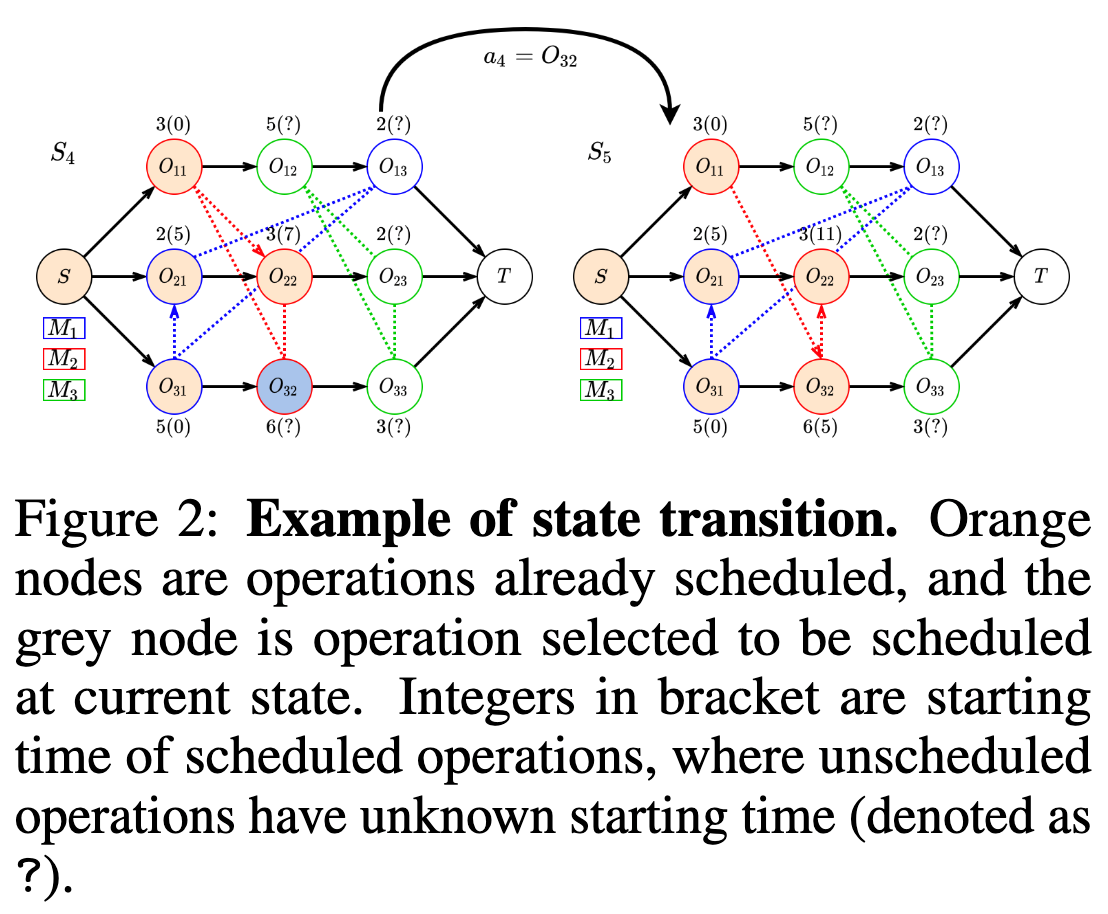
\includegraphics[width=\linewidth]{jssp_rl_state_transition_reference}
\caption{Illustrative graph state transition for sequential JSSP schedule construction.}
\label{fig:jssp_state_transition}
\end{figure}
% EN: This image remains a draft reference figure and should be redrawn in an original style or supported by a verified citation before submission.
% CN: 该图仍是参考草图，投稿前需要重绘为原创风格或补充核实过的引用。

\subsection{MDP Definition}
% EN: Be explicit about observation, action, reward, and transition. This is where the RL method becomes reproducible.
% CN: 明确定义 observation、action、reward 和 transition，这是强化学习方法可复现的关键。
\begin{addedblock}
The Markov decision process is defined over partial schedules. The agent does not directly command vehicle acceleration; instead, it constructs a discrete operation order that is later translated into time references for the smoother.
\end{addedblock}
\begin{itemize}
  \item \textbf{Observation}: graph features including operation status, estimated processing time, vehicle arrival time, route order, and conflict-zone occupancy.
  \item \textbf{Action}: selection of one schedulable operation, equivalent to assigning the next priority to a vehicle-zone traversal.
  \item \textbf{Transition}: update of the partial schedule after the selected operation is placed, including newly schedulable operations.
  \item \textbf{Reward}: negative schedule cost, such as incremental delay, makespan increase, stop penalty, infeasibility penalty, or a weighted combination of these terms.
\end{itemize}

\subsection{Offline Training and Online Rollout}
\begin{addedblock}
Let $\pi_\theta$ denote the trained RL policy. During offline training, the parameters $\theta$ are optimized using sampled JSSP/AIM instances and simulation feedback. During online deployment, $\theta$ is frozen. For a scheduling event at time $t$, the scheduler initializes the partial schedule with fixed commitments, computes the schedulable set, and repeatedly queries $\pi_\theta$ to select the next operation. The rollout terminates only when all remaining operations of the current active vehicles have been scheduled.

After the rollout produces a complete operation order, a deterministic schedule generator assigns target entry times $s_{i,k}$ and occupancy intervals using the selected order, route precedence constraints, fixed commitments, and estimated processing times $p_{i,k}$. The resulting reservation set $\mathcal{S}$ is then sent to the low-level smoother. Thus, the online stage is policy inference plus schedule generation, not online RL training.
\end{addedblock}

\subsection{Training Route}
% EN: Explain how training episodes are generated, how traffic demand changes, and how the learned policy is evaluated.
% CN: 说明 episode 如何生成、交通流如何变化、训练好的策略如何评估。
\begin{addedblock}
The training route is organized in three stages. First, an abstract JSSP/AIM high-level scheduler is trained on generated graph instances so that the policy learns to construct feasible and efficient operation orders independent of a specific microscopic simulator. Second, the trained scheduler is connected to SUMO for closed-loop validation or additional simulation-only fine-tuning under sampled traffic demand, routes, and arrival patterns. Third, the low-level smoother is introduced into the loop so that infeasible schedules, excessive stopping, and large tracking errors can be reflected in the reward or evaluation metrics.

This staged design separates learning from online control. Any fine-tuning with SUMO or smoother feedback is performed before deployment or during offline simulation experiments; the deployed intersection manager uses the trained policy for sequential rollout only.
\end{addedblock}

% CN summary for author review only; not visible in the compiled PDF:
% 训练建议：先训练抽象 JSSP/AIM high-level scheduler；再接入 SUMO 做 closed-loop fine-tuning 或验证；最后接 low-level smoother，并加入 infeasible penalty、stop penalty 和 tracking error 相关指标。在线部署时只做 policy rollout，不边训练边控制车辆。
% EN: Decide later whether the policy is graph neural network based, pointer-network based, or another architecture.
% CN: 后续需要确定策略网络结构，例如 GNN、pointer network 或其他图调度网络。

\section{Low-Level Trajectory Smoothing}
\label{sec:trajectory_smoothing}
% EN: This section bridges schedule and executable vehicle behavior. Define the smoother inputs, constraints, and output trajectory.
% CN: 本节连接抽象调度和车辆实际执行，需要定义平滑器输入、约束和输出轨迹。

The low-level controller converts scheduled conflict-zone entry times into feasible speed commands. Instead of stopping at the intersection and waiting for permission, a vehicle begins adjusting its speed upstream so that it reaches each conflict zone near the assigned time.

\subsection{Scheduled-Time Tracking}
% EN: Define tracking error between planned arrival time and assigned operation start time.
% CN: 定义车辆预计到达时间和调度开始时间之间的跟踪误差。
For vehicle $i$, let $\hat{t}_{i,k}$ denote the predicted arrival time at conflict zone $z_{i,k}$ under the current velocity plan. The tracking error is
\begin{equation}
  e_{i,k} = \hat{t}_{i,k} - s_{i,k}.
  \label{eq:tracking_error}
\end{equation}
The smoother penalizes large tracking errors while also discouraging excessive acceleration and jerk.

\subsection{Smooth Velocity Optimization}
% EN: Add the final barrier-function or optimization formulation here after the lower-level method is fixed.
% CN: 等低层方法确定后，在这里加入 barrier function 或优化问题的完整公式。
A generic smoothing objective can be written as
\begin{equation}
  \min_{\bm{u}_i} \sum_k w_t e_{i,k}^2 + \sum_h w_a a_i(h)^2 + \sum_h w_j j_i(h)^2,
  \label{eq:smoother_objective}
\end{equation}
subject to speed, acceleration, safety-distance, and conflict-zone time-window constraints. Here $\bm{u}_i$ denotes the control sequence, $a_i(h)$ is acceleration, and $j_i(h)$ is jerk at prediction step $h$.

\subsection{Barrier and Fallback Conditions}
% EN: Explain how safety is maintained when tracking fails or communication becomes unreliable.
% CN: 说明当跟踪失败或通信不可靠时如何保证安全。
Barrier-function constraints can be used to keep vehicles outside occupied conflict zones and preserve longitudinal safety. If the scheduled-time tracking problem becomes infeasible, the controller switches to a conservative fallback that stops before the intersection and requests a new high-level schedule.

% EN: Later, connect this section to energy consumption metrics and stop reduction in the experiments.
% CN: 后续实验中需要把本节和平滑性、停车次数、能耗代理指标联系起来。

\section{Experimental Setup}
\label{sec:experimental_setup}
% EN: Describe exactly how the method will be tested. This section should make the future results credible and reproducible.
% CN: 本节写清楚方法如何测试，让后续结果可信且可复现。

\subsection{Simulation Platform}
% EN: SUMO is the main training and evaluation platform. CARLA can be used later for vehicle-in-the-loop validation.
% CN: SUMO 作为主要训练和评估平台，CARLA 后续可用于 vehicle-in-the-loop 验证。
The first evaluation stage will be conducted in SUMO because it supports scalable microscopic traffic simulation and repeated training episodes. A later validation stage can connect the scheduler and smoother to CARLA to examine vehicle-level execution under richer dynamics and perception assumptions.

\subsection{Scenarios and Baselines}
% EN: Define intersection layouts, vehicle demand levels, and baseline controllers.
% CN: 定义路口布局、车流密度和对比基线。
The experiments will include multiple traffic densities and route distributions. The primary baseline is a first-come-first-served controller that requires vehicles to stop at the intersection stop line before crossing. Additional baselines may include heuristic priority rules and a scheduler without trajectory smoothing.

\begin{table}[!t]
\caption{Candidate Baseline Methods}
\label{tab:baselines}
\centering
\renewcommand{\arraystretch}{1.15}
\begin{tabular}{p{0.28\linewidth}p{0.58\linewidth}}
\toprule
\textbf{Method} & \textbf{Description} \\
\midrule
FCFS stop-line & Vehicles are served by arrival order and wait before entering the intersection. \\
Heuristic scheduler & Passing priority is selected by a handcrafted rule such as earliest arrival or shortest traversal time. \\
JSSP scheduler only & High-level schedule is used without low-level velocity smoothing. \\
Proposed hierarchy & JSSP/RL scheduler plus low-level smooth trajectory tracking. \\
\bottomrule
\end{tabular}
\end{table}

\subsection{Evaluation Metrics}
% EN: Report metrics that reflect both scheduling quality and vehicle-level execution quality.
% CN: 指标需要同时反映调度质量和车辆执行质量。
\begin{table}[!t]
\caption{Candidate Evaluation Metrics}
\label{tab:metrics}
\centering
\renewcommand{\arraystretch}{1.15}
\begin{tabular}{p{0.34\linewidth}p{0.52\linewidth}}
\toprule
\textbf{Metric} & \textbf{Purpose} \\
\midrule
Average delay & Measures traffic efficiency. \\
Throughput & Counts vehicles that clear the intersection per unit time. \\
Number of stops & Evaluates stop-and-go reduction. \\
Acceleration variance & Measures trajectory smoothness. \\
Energy proxy & Estimates energy-related cost from speed and acceleration profiles. \\
Computation time & Checks real-time scheduling feasibility. \\
\bottomrule
\end{tabular}
\end{table}

% EN: Later, add exact SUMO network files, route generation parameters, random seeds, and training hyperparameters.
% CN: 后续补充 SUMO 路网、route 生成参数、随机种子和训练超参数。

\section{Results and Discussion}
\label{sec:results_discussion}
% CN-SECTION: 结果讨论章节预留未来实验分析结构，避免在无数据时作强结论。
% EN: This is a placeholder structure for future experimental results. Keep the claims conservative until data is available.
% CN: 这里先放结果章节框架。在真实数据出来前，所有结论都要保守表达。

\subsection{Scheduling Performance}
% EN: Compare delay, throughput, and makespan against baselines.
% CN: 比较 proposed method 和 baselines 在延误、吞吐量、makespan 上的表现。
This subsection will report whether the learned JSSP scheduler improves intersection throughput and reduces delay under different traffic densities. The analysis should include both average performance and variability across random seeds.

\subsection{Trajectory Smoothness}
% EN: Show whether smoothing reduces stops and acceleration fluctuation.
% CN: 展示速度平滑是否减少停车次数和加速度波动。
This subsection will evaluate whether the low-level smoother reduces unnecessary stops before the intersection. Useful plots include speed-time profiles, acceleration-time profiles, and histograms of stop counts.

\subsection{Ablation Study}
% EN: Compare full hierarchy, scheduler only, smoother only if meaningful, and FCFS.
% CN: 做消融实验：完整框架、只有调度、只有平滑或 FCFS。
An ablation study should separate the contribution of high-level scheduling from that of low-level trajectory smoothing. The expected comparison is between the proposed hierarchy, the JSSP scheduler without smoothing, and the FCFS stop-line baseline.

\subsection{Limitations}
% EN: Discuss limitations honestly: communication assumptions, scalability, policy generalization, and sim-to-real gap.
% CN: 诚实讨论局限：通信假设、规模扩展、策略泛化和仿真到真实车辆的差距。
The current framework assumes reliable communication and known routes inside the management region. Future work should test robustness to delayed messages, uncertain vehicle dynamics, mixed traffic with human-driven vehicles, and deployment on vehicle-in-the-loop platforms.


\section{Conclusion}
\label{sec:conclusion}
% EN: Summarize the research idea and avoid claiming numerical improvements until experiments are complete.
% CN: 总结研究思路。在实验完成前不要声称具体数值提升。

This paper draft presents a hierarchical framework for autonomous intersection management that combines JSSP-based high-level scheduling with low-level smooth trajectory optimization. The core idea is to use reinforcement learning to construct efficient conflict-zone schedules while enabling vehicles to execute those schedules through advance speed adjustment rather than stop-line waiting. The planned evaluation will compare the proposed method against FCFS and heuristic baselines in SUMO, with future validation in CARLA. The long-term goal is to make graph-based intersection scheduling more executable for real connected autonomous vehicles.

\begin{addedblock}
A central implementation choice is that reinforcement learning is used for offline policy learning, whereas online intersection control uses the trained policy only for sequential schedule rollout. This distinction keeps the deployed scheduler focused on real-time inference: it orders the remaining operations of the active vehicles, generates target conflict-zone entry times, and relies on the smoother to confirm executable trajectories or request replanning.
\end{addedblock}

% CN summary for author review only; not visible in the compiled PDF:
% 结论需要再次强调：部署阶段不是持续在线训练 RL，而是使用已经训练好的 high-level policy 进行 online sequential rollout，并把生成的 order/target times 交给低层 smoother 执行与反馈。


\section*{Acknowledgment}
The author would like to thank collaborators and supervisors who provide feedback on the intersection management formulation, simulation design, and trajectory smoothing method.

\ifCLASSOPTIONcaptionsoff
  \newpage
\fi

\bibliographystyle{IEEEtran}
\bibliography{references}

\end{document}
